\documentclass[11pt]{article}


\usepackage{graphicx}
\usepackage{amsmath}
\usepackage{amssymb}
% \usepackage{txfonts}
\usepackage{mathtools}
\usepackage{pifont}
\usepackage{amsfonts}
\usepackage{enumitem}
% \usepackage{titlesec}
\usepackage{color}
\usepackage{xparse}
%\usepackage{subfigure}
\usepackage[hyphens]{url}
\usepackage[colorlinks,allcolors=darkred]{hyperref}
% \usepackage{caption}
\usepackage{subfigure}
\usepackage{tikz}
% \usepackage[none]{hyphenat}
% \usepackage{wrapfig}
% \usepackage{xparse}
\usepackage{tabularx}
% \usepackage{longtable,tabu}
\usepackage{multirow}
% \usepackage{booktabs}
\usetikzlibrary{patterns,arrows,decorations.markings}
\definecolor{darkblue}{rgb}{0.1,0.2,0.7}
\definecolor{darkred}{rgb}{0.7,0.2,0.1}
%\everymath{\displaystyle}
\everymath{\color{darkblue}}

\newcommand{\un}[1][]{u_h^{n#1}}
\newcommand{\bun}[1][]{\bar{u}_i^{n#1}}
\newcommand{\wn}[1][j]{w_h^{n,#1}}
\newcommand{\uh}[1][u]{{#1}_h}
\newcommand{\uref}[1][u]{{#1}_\textrm{ref}}
\newcommand{\tn}{t_n}
\newcommand{\tf}[1][n+1]{t_{#1}}
\newcommand{\xl}[1][i]{x_{#1-1}}
\newcommand{\xr}{\xl[i]}
\newcommand{\I}[1][i]{I_{#1}}
\newcommand{\intI}[1][\I]{\int_{#1}}
\newcommand{\intn}{\int_{t_n}^{t_{n+1}}}
\newcommand{\intdt}[1][]{\int_{0}^{#1\Delta{t}}}
\newcommand{\dt}[1][t]{\Delta{#1}}
\newcommand{\dx}[1][x]{\,\mathrm{d}{#1}}
\newcommand{\dydx}[2][x]{\frac{\mathrm{d}#2}{\mathrm{d}#1}}
%\newcommand{\cx}[1][n]{\check{x}^{#1}}
\newcommand{\cx}[1][]{X^{n#1}}
\newcommand{\cxt}[2][]{\cx[#1](#2;x)}
% \newcommand{\cxt}[2][,j]{\cx[#1](#2;x)}
%\newcommand{\cxt}[2][x]{\cx[n,j](#2;#1)}
\newcommand{\xt}[1][t]{\cx(#1;x)}
\newcommand{\xs}[1][x]{#1^*}
%\newcommand{\xt}[1][t]{\cxt{#1}}
% \newcommand{\cI}[1][x]{\mathcal{K}_j(#1)}
\newcommand{\cI}[1][x]{\mathcal{I}_n(#1)}
\NewDocumentCommand{\St}{O{t} O{n} O{S}}{#3_{\hspace{-2pt}#2}(#1)}
% \newcommand{\St}[1][t]{S\hspace{-1pt}(#1)}
% \newcommand{\St}[1][t]{S_{#1}}
\newcommand{\Sdt}[1][j]{S_{\hspace{-2pt}#1}(\tau)}
% \newcommand{\Sdt}[1][j]{S_{\tau}^{#1}}
\newcommand{\Vh}[1][q]{V_h^#1}
\newcommand{\Pk}{\mathbb{P}_q}
\newcommand{\R}[1][]{\mathbb{R}^{#1}}
\newcommand{\vl}[1][v]{{#1}^+}
\newcommand{\vr}[1][v]{{#1}^-}
\newcommand{\vlr}[1][v]{{#1}^\mp}
\newcommand{\vs}[1][s]{\varphi_{#1}}
\newcommand{\uhl}[1][n,]{u_h^{#1-}}
\newcommand{\uhr}[1][n,]{u_h^{#1+}}
%\newcommand{\w}[1][r]{\omega_{#1}}
\newcommand{\sumk}[1][j-1]{\sum_{k=0}^{#1}}
\newcommand{\sumq}{\sum_{r=0}^{q}}
\NewDocumentCommand{\gsum}{O{} O{} O{}}{\sum_{#1=#2}^{#3}}
% \newcommand{\ajk}[1][\alpha]{{#1}_{j,k}}
\NewDocumentCommand{\ajk}{O{j,k} O{\alpha}}{{#2}_{#1}}
% \newcommand{\cjk}{\ajk[\tilde{\alpha}]}
% \newcommand{\bjk}{\ajk[\tilde{\beta}]}
\newcommand{\cjk}[1][j,k]{\ajk[#1][\alpha]}
\newcommand{\bjk}[1][j,k]{\ajk[#1][\beta]}
\newcommand{\Th}[1][M]{\mathcal{T}_h^{#1}}
% \newcommand{\Ltw}[1][2]{L$_#1$}
% \newcommand{\Ltw}[1][$]{L#1_2#1}
% \NewDocumentCommand{\Ltw}{O{$} O{2}}{L#1_2#1}
\newcommand{\xk}[1][r]{\xl[#1]}
%\newcommand{\cxk}[1][x]{\cx[j](#1)}
\newcommand{\cxk}[1][]{\check{X}^{n#1}(x)}
\newcommand{\wk}[1][r]{\omega_{#1}}
\newcommand{\Ol}{\alpha}
\newcommand{\Or}{\beta}
%\newcommand{\wnb}[1][j]{\mathbf{w}^{(#1)}}
%\newcommand{\unb}[1][]{\mathbf{u}^{n#1}}
\newcommand{\wnb}[1][j]{\mathbf{w}^{(#1)}}
\newcommand{\unb}[1][]{\mathbf{u}^{n#1}}
\newcommand{\Lh}[1][\Delta{t}]{\mathbf{L}_h^{#1}}
\newcommand{\Rh}{\mathbf{R}_h}
\newcommand{\jump}[1]{\ensuremath{[\![#1]\!]}}
%\newcommand{\Qj}[1][j]{\mathcal{E}_{#1}}
\newcommand{\Qj}[1][\Delta{t}]{L_h^{#1}}
\newcommand{\Rj}[1][R]{#1_h}
\newcommand{\tmath}[2][\hspace{1ex}]{\text{\color{black}#2#1}}
\newcommand{\sbrace}[2][\,]{\left(#1#2#1\right)}
\newcommand{\cbrace}[2][\,]{\left\{#1#2#1\right\}}
\newcommand{\dbrace}[2][\,]{\left[#1#2#1\right]}
\newcommand{\abs}[2][\,]{\left|#1#2#1\right|}
\newcommand{\order}[2][~]{\mathcal{O}\left({#2}^{#1}\right)}

\newcommand{\norm}[2][]{\left\Arrowvert\, #2\, \right\Arrowvert_{#1}}
\newcommand{\centralize}[1][2mm]{\rule[#1]{0pt}{2mm}\rule[-#1]{0pt}{2mm}}

\tikzset{middlearrow/.style={
            decoration={markings,
              mark= at position 0.5 with {\arrow[scale=2]{#1}} ,
          },
        postaction={decorate}
      }
}

\title{
  SLDG integration following Qiu et al. 2011
}


% \setlength{\parindent}{8mm}
\setlength{\parskip}{2mm}

% \setmainfont{Times New Roman}
% 
% \newcommand{\co}{CO$_2$~}

\begin{document}

\maketitle

Consider a partition of the domain $I = \dbrace{\Ol,\Or}$ into subintervals $\I = \dbrace{\xl,\xr},\quad i = 1,\ldots,N$ such that
\begin{align*}
  \Ol = x_0 < x_1 < \cdots < x_N = \Or.
\end{align*}

We assume that $\xs = \cxk$ is the foot of the characteristic reaching a fixed node $x\in\I[j]$ at time $\tau = \dt$, so that
%
\begin{align*}
  \cxk \coloneqq \cxt{0} = x - \intdt a_n(\cxt{\tau})\dx[\tau].
\end{align*}
%
%
%
\begin{figure}[!b]%[htbp]
  \centering
% \input{xticTrace}
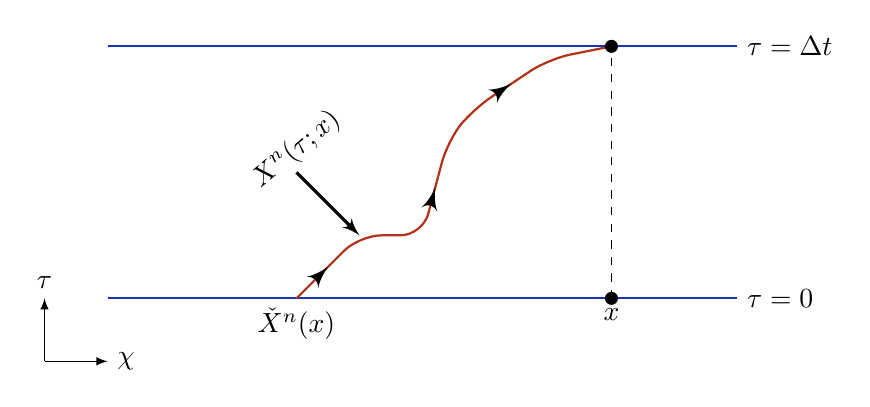
\begin{tikzpicture}[scale=0.8]
\coordinate (O) at (0,0);
\coordinate (A) at (10,0);
\coordinate (B) at (0,4);
\coordinate (C) at (10,4);
\coordinate (D) at (8,0);
\coordinate (E) at (8,4);
\coordinate (F) at (3,0);
\node[] () at (C)[right] {$\tau = \dt$};
\node[] () at (A)[right] {$\tau = 0$};
\node[] () at (D)[below] {$x$};
\node[] () at (F)[below] {$\cxk$};
\draw[darkblue,thick] (O) -- (A);
\draw[darkblue,thick] (B) -- (C);
\draw[dashed] (D) -- (E);
\draw[thick, draw=darkred, rounded corners=8pt] (F) to (4,1) to (5,1) to (5.4,2.5) to (5.8,3) to (7,3.8) to (E);
\draw[->, >=latex',very thick] (3,2) to (4,1);
\path[middlearrow={latex'}] (5,1) to (5.4,2.5);
\path[middlearrow={latex'}] (F) to (4,1);
\path[middlearrow={latex'}] (5.8,3) to (7,3.8);
\node[] () at (3,1.5)[left,above] {\rotatebox[origin=c]{40}{$\cxt{\tau}$}};
\node[circle, fill, scale=0.5] () at (D) {};
\node[circle, fill, scale=0.5] () at (E) {};
\draw[->,>=latex] (-1,-1) to  (-1,0) node[above]{$\color{black}\tau$};
\draw[->,>=latex] (-1,-1) to  (0,-1) node[right]{$\chi$};
\end{tikzpicture}
\caption{Illustration of the characteristic curve $\cxt{\tau}$, characteristic foot $\cxk$ and trace interval $\cI = \left[\cxk,x\right]$.}
\label{trace:fig}
\end{figure}
%
Define the trace interval $\cI$ for a fixed node $x\in\I[j]$ by (see Figure \ref{trace:fig})
%
\begin{align*}
  \cI \coloneqq \left[x,\cxk\right] \cup \left[\cxk,x\right].
\end{align*}
%
We want to evaluate the following integral:
%
\begin{align}\label{Lh:def}
  \Qj(\un(x)) &= \intdt a(x,\tau)\St[\tau]\un(x)\dx[\tau] = \int_{\cxk}^{x}\un(\xi)\dx[\xi]\notag \\
 &= \text{sign}\,\left(x-\cxk\right)\sum_{k=1}^M\int_{\cI\,\cap\,\I[k]}\un(\xi)\dx[\xi]
 \end{align}
%
 Let
 \begin{align*}
   L \coloneqq \abs{I} = x_N - x_0 = \Or - \Ol.
 \end{align*}

 Assume periodic boundary conditions. Then we have two important assumptions to make.

\begin{enumerate}
  \item[Assumption L.] $\xs \leq x$.
    \begin{enumerate}
      \item[\bfseries Case 1.] $x_0 \leq \xs\leq x_N$:\\
        If $\xs\in\I$, then $i\leq j$.
        \begin{align*}
          \Qj\un(x) &= \int_{\xs}^x\un(\xi)\dx[\xi]\\
          &= \int_{\xs}^{x_i}\un(\xi)\dx[\xi] + \int_{x_i}^{x_{j-1}}\un(\xi)\dx[\xi] + \int_{x_{j-1}}^x\un(\xi)\dx[\xi]\qquad (i < j)
        \end{align*}
      \item[\bfseries Case 2.] $\xs < x_0$:
        \begin{align*}
          \Qj\un(x) &= \int_{\xs}^x\un(\xi)\dx[\xi]\\
          &= \int_{x_0}^{x}\un(\xi)\dx[\xi] + \int_{\xs[y]}^{x_N}\un(\xi)\dx[\xi] + k\int_{x_0}^{x_N}\un(\xi)\dx[\xi]\\
          &= \int_{\xs[y]}^{x_N}\un(\xi)\dx[\xi] + (k+1)\int_{x_0}^{x_N}\un(\xi)\dx[\xi],
          \intertext{where}
          & \xs[y] = x_N - \sbrace{(x_0-\xs)\text{ mod } L} \in \dbrace{x_0, x_N},\\
          & k = (x_0-\xs)\text{div}L \in \mathbb{N}
        \end{align*}
        If $\xs[y]\in\I$ and $i\leq j$, then Case 1 can be used to evaluate the integral over $\dbrace{\xs[y],x}$,
        otherwise we use Case 1 of Assumption R. Remark also that if $i=j$, Case 1 becomes
        $\Qj\un(x) =  \int_{\xs}^x\un(\xi)\dx[\xi]$.
    \end{enumerate}
  \item[Assumption R.] $\xs \geq x$.
    \begin{enumerate}
      \item[\bfseries Case 1.] $x_0 \leq \xs\leq x_N$:\\
        If $\xs\in\I$, then $i\geq j$.
        \begin{align*}
          \Qj\un(x) &= -\int_x^{\xs}\un(\xi)\dx[\xi]\\
          &= -\dbrace{\int_{x}^{x_j}\un(\xi)\dx[\xi] + \int_{x_j}^{x_{i-1}}\un(\xi)\dx[\xi] + \int_{x_{i-1}}^{\xs}\un(\xi)\dx[\xi]}\quad (i > j)
        \end{align*}
        In this case it suffices to reverse the roles of $\xs\longleftrightarrow x$, apply Case 1 of Assumption L and tag a minus sign to the result.
      \item[\bfseries Case 2.] $\xs > x_N$:
        \begin{align*}
          \Qj\un(x) &= -\int_x^{\xs}\un(\xi)\dx[\xi]\\
          &= -\dbrace{\int_{x}^{x_N}\un(\xi)\dx[\xi] + \int_{x_0}^{\xs[y]}\un(\xi)\dx[\xi] + k\int_{x_0}^{x_N}\un(\xi)\dx[\xi]}\\[2ex]
          &= \int_{\xs[y]}^{x_N}\un(\xi)\dx[\xi] - (k+1)\int_{x_0}^{x_N}\un(\xi)\dx[\xi],
          \intertext{where}
          & \xs[y] = x_0 + \sbrace{(\xs-x_N)\text{ mod } L},\\
          & k = (\xs-x_N)\text{ div } L.
        \end{align*}
    \end{enumerate}
\end{enumerate}




\end{document}
